
%(BEGIN_QUESTION)
% Copyright 2011, Tony R. Kuphaldt, released under the Creative Commons Attribution License (v 1.0)
% This means you may do almost anything with this work of mine, so long as you give me proper credit

Suppose the lamp refuses to light up.  A voltmeter registers 24 volts between test points {\bf C} and {\bf D}:

$$\includegraphics[width=15.5cm]{i01746x01.eps}$$

First, list all the possible (single) faults that could account for all measurements and symptoms in this circuit, including failed wires as well as failed components:

\vskip 50pt

Now, determine the diagnostic value of each of the following tests, based on the faults you listed above.  If a proposed test could provide new information to help you identify the location and/or nature of the one fault, mark ``yes.''  Otherwise, if a proposed test would not reveal anything relevant to identifying the fault (already discernible from the measurements and symptoms given so far), mark ``no.''

% No blank lines allowed between lines of an \halign structure!
% I use comments (%) instead, so that TeX doesn't choke.

$$\vbox{\offinterlineskip
\halign{\strut
\vrule \quad\hfil # \ \hfil & 
\vrule \quad\hfil # \ \hfil & 
\vrule \quad\hfil # \ \hfil \vrule \cr
\noalign{\hrule}
%
% First row
{\bf Diagnostic test} & {\bf Yes} & {\bf No} \cr
%
\noalign{\hrule}
%
% Another row
Measure $V_{CF}$ &  &  \cr
%
\noalign{\hrule}
%
% Another row
Measure $V_{ED}$ &  &  \cr
%
\noalign{\hrule}
%
% Another row
Measure $V_{AB}$ &  &  \cr
%
\noalign{\hrule}
%
% Another row
Measure $V_{AD}$ &  &  \cr
%
\noalign{\hrule}
%
% Another row
Measure $V_{CB}$ &  &  \cr
%
\noalign{\hrule}
%
% Another row
Measure $V_{EF}$ &  &  \cr
%
\noalign{\hrule}
%
% Another row
Measure current through wire connecting {\bf A} and {\bf C} &  &  \cr
%
\noalign{\hrule}
%
% Another row
Jumper {\bf A} and {\bf C} together &  &  \cr
%
\noalign{\hrule}
%
% Another row
Jumper {\bf B} and {\bf D} together &  &  \cr
%
\noalign{\hrule}
%
% Another row
Jumper {\bf A} and {\bf B} together &  &  \cr
%
\noalign{\hrule}
} % End of \halign 
}$$ % End of \vbox

Finally, develop a rule you may use when assessing the value of each proposed test, based on a comprehensive list of possible faults.


\vskip 20pt \vbox{\hrule \hbox{\strut \vrule{} {\bf Suggestions for Socratic discussion} \vrule} \hrule}

\begin{itemize}
\item{} Identify which fundamental principles of electric circuits apply to each step of your analysis of this circuit.  In other words, be prepared to explain the reason(s) ``why'' for every step of your analysis, rather than merely describing those steps.
\item{} Suppose the fault were intermittent: sometimes the lamp lights up, and other times it goes out.  Explain how you could use a digital multimeter (DMM) set to {\it record} voltage as a troubleshooting tool to determine where the fault is located in the circuit over a span of time too long for you to personally observe the circuit.
\end{itemize}

\underbar{file i01746}
%(END_QUESTION)





%(BEGIN_ANSWER)

Here is a comprehensive list of faults, each one individually capable of accounting for the symptom (no light) and the measurement of 24 volts between {\bf C} and {\bf D}:

\begin{itemize}
\item{} Lamp burned out (failed open)
\item{} Wire failed open between {\bf A} and {\bf C}
\item{} Wire failed open between {\bf B} and {\bf D}
\end{itemize}

Based on this short list of possible faults -- assuming only {\it one} of them is actually true -- the value of each proposed test is as follows:

% No blank lines allowed between lines of an \halign structure!
% I use comments (%) instead, so that TeX doesn't choke.

$$\vbox{\offinterlineskip
\halign{\strut
\vrule \quad\hfil # \ \hfil & 
\vrule \quad\hfil # \ \hfil & 
\vrule \quad\hfil # \ \hfil \vrule \cr
\noalign{\hrule}
%
% First row
{\bf Diagnostic test} & {\bf Yes} & {\bf No} \cr
%
\noalign{\hrule}
%
% Another row
Measure $V_{CF}$ &  & $\surd$ \cr
%
\noalign{\hrule}
%
% Another row
Measure $V_{ED}$ &  & $\surd$ \cr
%
\noalign{\hrule}
%
% Another row
Measure $V_{AB}$ & $\surd$ &  \cr
%
\noalign{\hrule}
%
% Another row
Measure $V_{AD}$ & $\surd$ &  \cr
%
\noalign{\hrule}
%
% Another row
Measure $V_{CB}$ & $\surd$ &  \cr
%
\noalign{\hrule}
%
% Another row
Measure $V_{EF}$ &  & $\surd$ \cr
%
\noalign{\hrule}
%
% Another row
Measure current through wire connecting {\bf A} and {\bf C} &  & $\surd$ \cr
%
\noalign{\hrule}
%
% Another row
Jumper {\bf A} and {\bf C} together & $\surd$ &  \cr
%
\noalign{\hrule}
%
% Another row
Jumper {\bf B} and {\bf D} together & $\surd$ &  \cr
%
\noalign{\hrule}
%
% Another row
Jumper {\bf A} and {\bf B} together &  & $\surd$ \cr
%
\noalign{\hrule}
} % End of \halign 
}$$ % End of \vbox

A good rule to apply when evaluating proposed tests is to ask the question: ``Will this test give me the exact same result no matter which one of the possible faults is true?''  If so, the test is useless.  If not (i.e. the results would differ depending on which of the possible faults was true), then the test has value because it will help narrow the field of possibilities.

%(END_ANSWER)





%(BEGIN_NOTES)

The fact we measure 24 VDC between points C and D tells us the wiring between those points and the voltage source is good.  Therefore, any test checking for power farther toward the source is a wasted step.  We also know that the problem cannot be a short, because otherwise we would not measure full supply voltage between points C and D.  Therefore, any diagnostic test checking for a short-circuit (e.g. current measurement) is futile.

%INDEX% Troubleshooting review: electric circuit diagnostic test usefulness (introduction to the concept)

%(END_NOTES)


